\documentclass[a4paper,12pt]{article}
\usepackage{graphicx}
\usepackage{float}
\usepackage{fancyhdr}
\usepackage{listings}
\lstset
{
  numbers=left,
  breaklines=true,
}
\pagestyle{fancy}
\rhead{Dane Johnson}
\title{CS-456 Project 3}
\author{Dane Johnson}
\date{April 18st, 2018}
\headheight=15pt
\begin{document}
\maketitle
\newpage
\section{Motivation}

This project was an attempt to demonstrate multiple ways of solving an NP-complete problem and to show to pros and cons
of each method as well as a way to demonstrate an example of an approximation algorithm and discuss when an approximation
would be useful and appropriate.

\section{Algorithms}
\subsection{Brute Force}
\subsubsection{Pseudocode}
\begin{lstlisting}[mathescape=true]
proc brute_force(G, s)
  for cycle in permute(G.V - {s})
    if len([s] + cycle + [s]) < min_cycle
      min_cycle $\gets$ [s] + cycle + [s]
  return min_cycle
proc permute(V)
  if len(V) == 1
    return V
  for u in V
    for permutation in permute(V - {u})
      permutations $\gets$ permutations + {permutation + {u}}
  return permutations
\end{lstlisting}
\subsubsection{Time Complexity}
This algorithm finds the shortest Hamiltonian Cycle by looking through every possible arrangement of nodes and determining which of them has the shortest distance. In order to accomplish this, the {\it permute} procedure creates all possible orderings of the nodes, an operation which takes $O(n!)$ time.
\subsubsection{Correctness Proof}
\begin{description}
\item [Invariant: ] After the $k$th iteration, $k$ cycles will have been considered for the shortest Hamiltonian cycle, and the minimum will be recorded.
\item [Initialization: ] $k$ is 0 initially, no paths have been considered and no shortest has been selected.
\item [Maintenance: ] After the $k$ iterations, the $k$th cycle is considered and, if it is the minimum yet considered, it is recorded.
\item [Termination: ] When the loop terminates, $k = n$, so all possible cycles have been considered and the minimum cycle has been recorded.
\end{description}
\subsubsection{Empirical Validation}
\begin{figure}[H]
  \centering
  \textbf{Brute Force}\par\medskip
  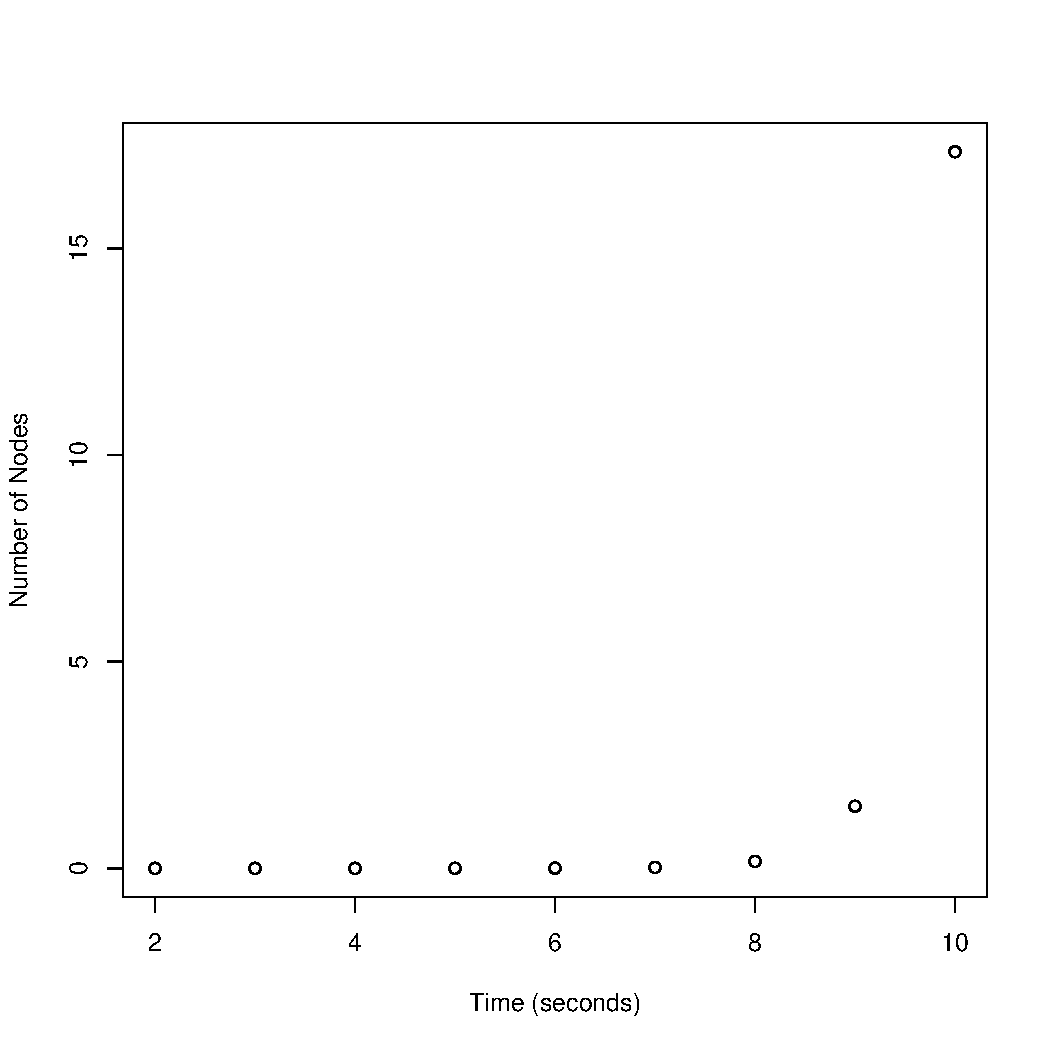
\includegraphics[width=1\linewidth]{BruteForce.pdf}
\end{figure}
Y axis in log scale.
\subsubsection{Observations}
Here we can see the data on a y-log graph. Even on a log graph, which would show polynomial relations as a straight line, we can still see a clear curvature. This would indicate that the time complexity of the algorithm is non-polynomial. Additionally, we can see that the algorithm begins to perform extremely poorly even at 10 nodes, taking a whole 17 seconds. 
\subsection{Branch and Bound}
\subsubsection{Pseudocode}
\begin{lstlisting}[mathescape=true]
proc branch-and-bound(G, s)
  state.placed $\gets$ {s}
  state.remaining $\gets$ G.V - {s}
  state.lower_bound $\gets$ lower_bound(state.placed, state.remaining)
  Q $\gets$ {state}
  while Q $\neq \emptyset$
    curr $\gets$ Q.extract_min()
    if curr is a solution
      if curr < solution
        solution $\gets$ curr
        prune Q for lower bounds < curr
    else
      Q $\gets$ Q + {next_states(curr)}
  return solution
proc next_states(state)
  next_states $\gets \emptyset$
  for $\forall u \in state.remaining$
    next_state.placed $\gets$ state.placed + {u}
    next_state.remaining $\gets$ state.remaining - {u}
    next_state.lower_bound $\gets$ lower_bound(next_state.placed, next_state.remaining)
    next_states = next_states + {next_state}
  return n
proc lower_bound(placed, remaining)
  add cost of all placed connections and cheapest edges from unplaced edges
\end{lstlisting}
\subsubsection{Time Complexity}
If the prune step is removed, this algorithm will generate the entire search tree, which will cause the algorithm to become a scan of the entire solution space. Given that, in the worst case, no pruning occurs, worst case time complexity for the algorithm is still $O(n!)$.
\subsubsection{Correctness Proof}
\begin{description}
\item [Invariant: ] At the end of the $k$th loop, $k$ nodes of the search tree have been explored.
\item [Initialization: ] Initially, $k = 0$, and only the source node is on the tree 
\item [Maintenance: ] Each step, all children of the most promising node are added to the tree to be explored, and the $k$th most promising node has been explored
\item [Termination: ] After $n!$ iterations, $n!$ options have been explored and the search tree has been completely explored.
\end{description}
\begin{figure}[H]
  \centering
  \textbf{Branch and Bound}\par\medskip
  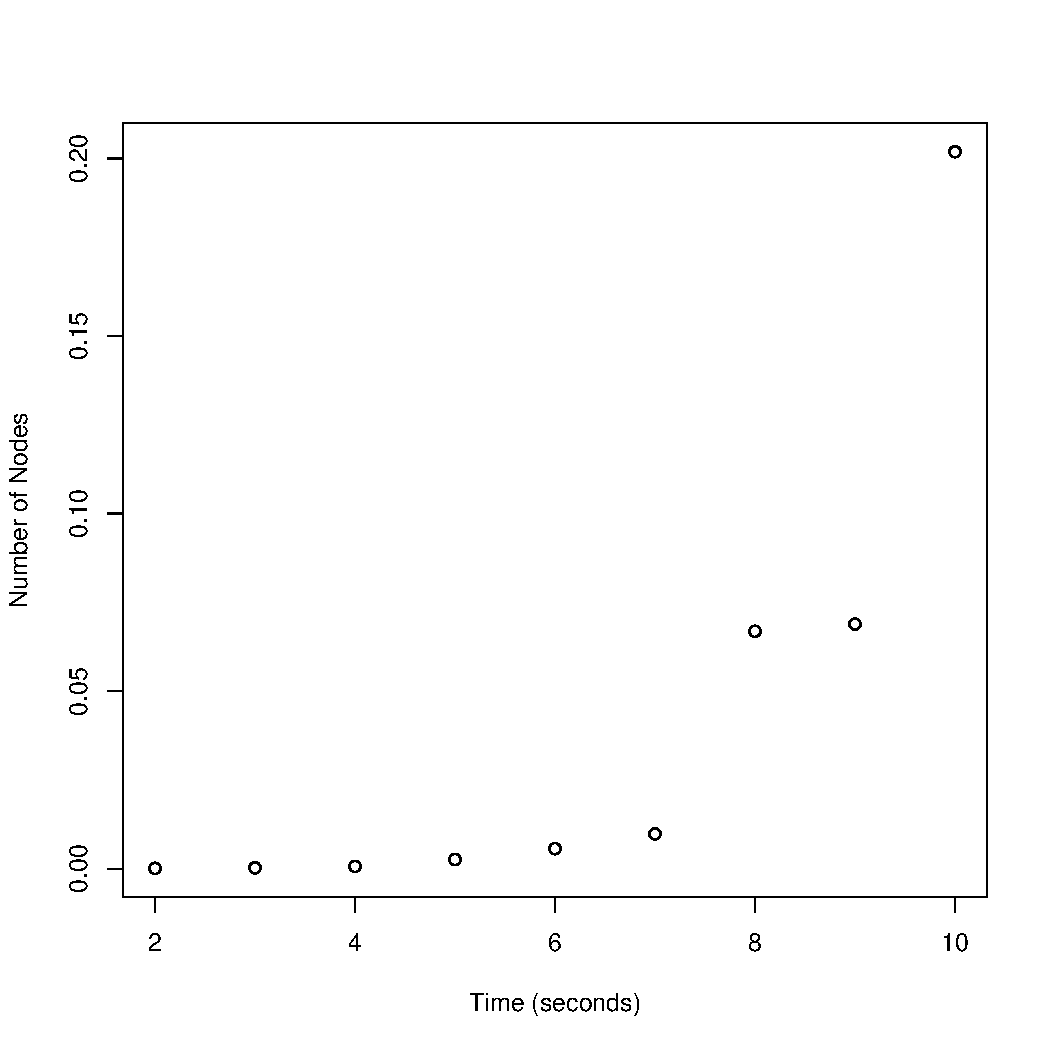
\includegraphics[width=1\linewidth]{BranchAndBound.pdf}
\end{figure}
Y axis in log scale.
\subsection{Observations}
Here we can again see a curvature on the y-log graph, which indicates a non-polynomial relationship. In this case, we can see the curve is less steep, indicating that the pruning element of the branch and bound algorithm is speeding up the search. This is also shown by the fact that a 10 node TSP can be solved in two-tenths of a second with branch and bound, whereas a brute force approach on the same graph takes 17 seconds. However, one weakness of the branch and bound approach is the need to find a good most promising node, and in cases like the 8 node TSP where the optimal path is not obvious, the algorithm can take much more time than average.
\subsection{Dynamic Programming}
\subsubsection{Pseudocode}
\begin{lstlisting}[mathescape=true]
proc dynamic_programming(G, s)
  cost $\gets \emptyset$
  for i in G.V - {s}
    cost({s, i}, i) = dist(s, i)
  for n - 2
    for i in G.V - {s}
      for $\forall$ n - 1 sized subsets S where $i \notin S$
        cost(S + {i}, i) = min{cost(S, j) + dist(j, i)} where $j \neq s, j \neq i, j \in S$
  return min{cost(S, i) + dist(i, s)} where $|S| = n$    
\end{lstlisting}
\subsubsection{Time complexity}
In order to generate all subsets of size $n$ ending at all points that are not the source, all $n - 1$ subsets ending at all points that are not the source must be generated. This creates the recurrance relation $T(n) = nT(n - 1) + c$, which expands to $T(n) = n((n - 1)T(n - 2) + d) + c$, which eventually exands to $1 * 2 * 3 * ... * (n - 1) * n + C = n!$, so the time complexity of this algorithm is still $O(n!)$ 
\subsubsection{Correctness Proof}
\begin{description}
\item [Invariant: ] After the $k$th iteration of the loop, all $k + 2$ subsets ending in $i$ have been generated.
\item [Initialization: ] Before the loop all 2 length subsets are generated.
\item [Maintenence: ] On each loop iteration, each $k + 2$ subset ending in each of $n$ is generated.
\item [Termination: ] When the loop terminates, $k = n - 2$, so all $n$ length subsets ending in $i  \forall  i  \in  n$ have been generated, and the minimum can be selected.
\end{description}
\begin{figure}[H]
  \centering
  \textbf{Dynamic Programming}\par\medskip
  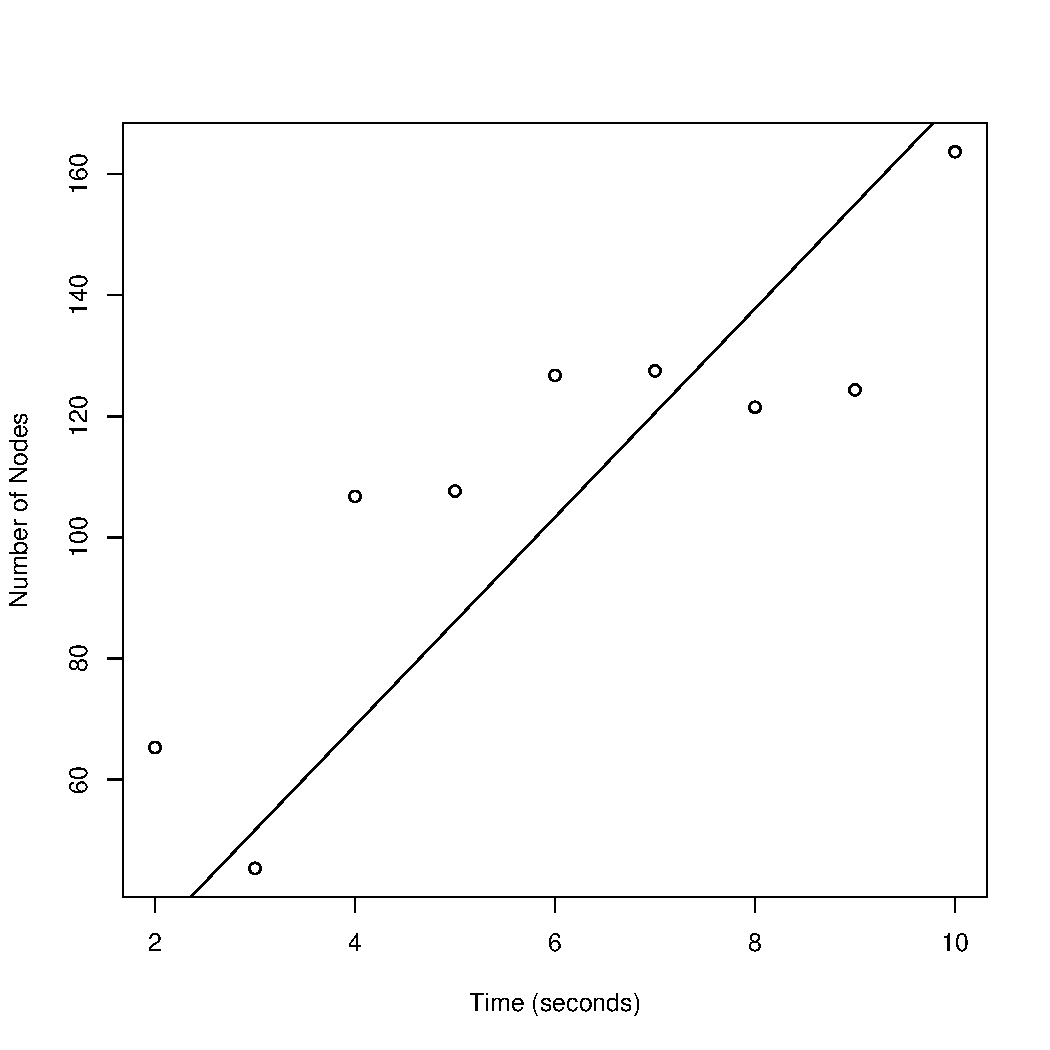
\includegraphics[width=1\linewidth]{DynamicProgramming.pdf}
\end{figure}
Y axis in log scale.
\subsection{Observations}
In the dynamic programming example, we can see a very nearly straight line on the y-log graph, however attempting to draw a straight edge reveals a slight curveture, indicating that the graph is still exponential. This graph does not have the same amount of variation that the branch and bound algorithm would have, as the bound on this algorithm is tighter, the same number of calculations are performed on all graphs of the same size, so the data are more regular.
\section{MST Approximation}
\subsection{Pseudocode}
\begin{lstlisting}[mathescape=true]
proc mst_approximation(G, s)
  for $\forall$ u in G.V
    d[u] $\gets$ $\infty$
  d[s] $\gets$ 0
  Q $\gets \emptyset$
  for $\forall$ u in G.V
    Q.insert(u)
  path $\gets emptyset$
  while Q $\neq \emptyset$
    u $\gets$ Q.extract_min()
    path $\gets$ path + {u}
    for $\forall (u, v) \in G.E$
      if d[v] < dist(u, v)
        d[v] = dist(u, v)
        q.decrease_key(v)
  return path + {s}
\end{lstlisting}
\subsection{Time Complexity}
Time complexity of the algorithm depends on the data structure used for $Q$, assuming a Min Priority Heap is used, time complexity will be as follows. Initializing the Q will take $\Theta(|V|)$ time, exploring each vertex takes $V$ time, extracting a minimum takes $lg(V)$ time, and each edge is replaxed exactly once, which indicates $O(E)$ time. Thus, the runtime of the algorithm is $O(E \times lg(v))$ time.
\subsubsection{Correctnesss Proof}
\begin{description}
\item [Invariant: ] At the start of each loop, the shortest path to every vertex that has been removed from $Q$ has been found and a completion order up to the last vertex has been recorded..
\item [Initialization: ] Initially, no elements have been removed from $Q$, so the invariant is trivially proven.
\item [Maintenence: ] On each loop iteration, the number of explored elements is incremented, and by selecting the vertex closest to the source not in the explored space, we know that the shortest path to that vertex must be through its parent in the explored space. Additionally, the path to the vertex has been recorded.
\item [Termination: ] When the loop terminates, every vertex has been removed from $Q$, and by the invariant, the shortest path to every vertex is known, and the discovery order has been fully recorded.
\end{description}
\subsection{Empirical Validation}
\begin{figure}[H]
  \centering
  \textbf{MST Approximation}\par\medskip
  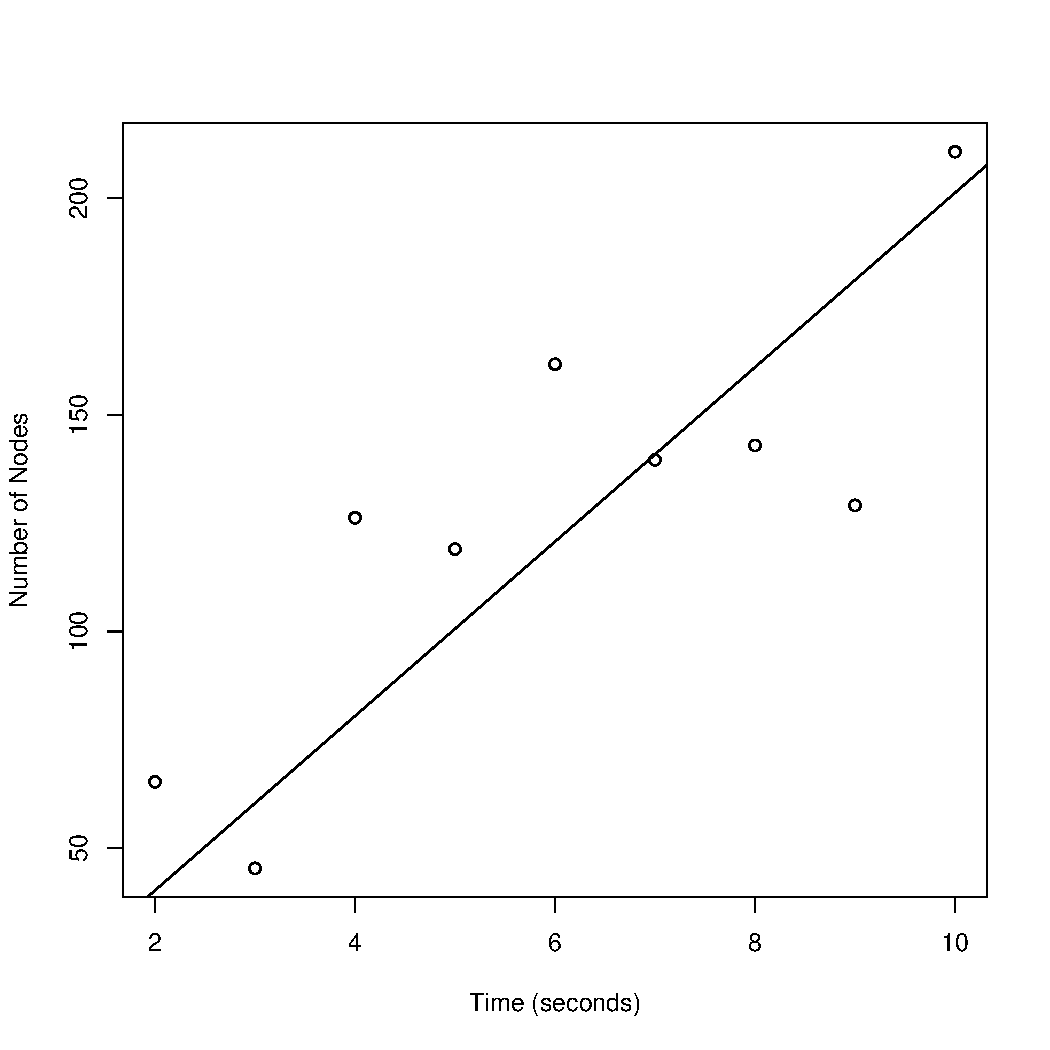
\includegraphics[width=1\linewidth]{MSTApproximation.pdf}
\end{figure}
Y axis in log scale.
\subsection{Observations}
The graph, again on a y-log scale, shows curvature, but a key difference here is that the concavity is downwards. This indicates a polynomial time relation, as hypothesized above. There are significant fluctuations in completion time, however in this algorithm that is likely to do with the clustering of data points, more clustered data points result in more comparisons needed to update keys, which results in variation in completion time.
\section{Conclusion}
\end{document}
